\chapter{Einführung in die Welt des Arduino: Digitale Ausgänge und Eingänge}

Der Arduino ist ein Mikrocontroller, der vom italienischen Professor Massimo Banzi entwickelt wurde, damit seine Studenten im Bereich \emph{Design} eine einfach zugängliche Möglichkeit fanden, Elektronik für künstlerische Projekte zu nutzen. Die vorgenommenen Vereinfachungen in der Handhabung von Mikrocontrollern gefielen jedoch nicht nur den Studenten von Massimo Banzi, sondern auch zahlreichen Studenten anderer Fachrichtungen, Schülern, Hobby-Elektronikern und sogar Fachleuten in der Industrie, sodass der Arduino rasch eine weltweite Verbreitung fand.

\bigskip
In diesem Kapitel lernst du\dots
\begin{itemize}
	\item \dots wie der Arduino aufgebaut ist,
	\item \dots wie man den Arduino mit dem PC verbindet und mit mBlock programmiert,
	\item \dots die digitalen Pins als Ausgänge zu benutzen, um eine LED zu steuern,
	\item \dots Schaltungen auf dem Steckbrett aufzubauen,
	\item \dots Widerstand, Spannung und Stromstärke im Stromkreis zu berechnen,
	\item \dots Widerstandsringe abzulesen, um die Größe des Widerstands zu bestimmen,
	\item \dots eine RGB-LED und eine 7-Segmentanzeige zu steuern,
	\item \dots das elektrische Potential an einem digitalen Pin einzulesen und \dots
	\item \dots mit Hilfe des elektrischen Potentials den Zustand eines Tasters abzufragen.
\end{itemize}

\begin{projektueberblick}
	\item Ampel \dotfill \pageref{proj:ampel}
	\item Augentestgerät \dotfill\pageref{proj:augentest}
	\item Farbenspektakel mit RGB-LED \dotfill\pageref{proj:rgbled1}
	\item Raketencountdown \dotfill\pageref{proj:raketencountdown}
	\item Fußgängerampel \dotfill\pageref{proj:fussampel}
	\item Juke-Box \dotfill\pageref{proj:jukebox}
\end{projektueberblick}

\section{Der Aufbau des Arduino UNO}
Mit der Zeit entwickelten sich zahlreiche andere Modelle des Arduino, die kleiner oder größer waren, über mehr oder weniger Anschlüsse verfügten, schneller oder langsamer waren usw. Das Standardmodell ist heute der Arduino Uno, den auch wir verwenden.

\begin{figure}[h]
	\centering
	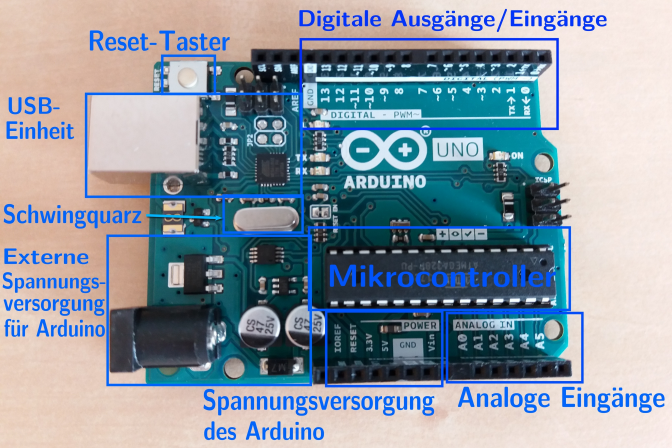
\includegraphics[width=0.8\textwidth]{pics/arduino-beschriftet.png}
	\caption{Die wichtigsten Komponenten eines Arduino Uno.}
	\label{abb:arduino-beschriftet}
\end{figure}

Abbildung \ref{abb:arduino-beschriftet} zeigt die wichtigsten Komponenten des Arduino Uno. Eine genauere Beschreibung dieser Funktionseinheiten und ihrer spezifischen Eigenschaften findet sich in Anhang \ref{sec:ueberblick}. Wichtig sind an dieser Stelle vor allem folgende Punkte:
\begin{itemize}
	\item Über den USB-Anschluss und das mitgelieferte Kabel lässt sich der Arduino mit dem PC verbinden und programmieren.
	\item Das Programm läuft nach dem Übertragen auf dem eigentlichen Mikrocontroller, dem langen schwarzen Ding in der Mitte. Der ganze Rest auf dieser kleinen Platine dient der einfacheren Handhabung des Mikrocontrollers.
	\item An den Seiten befinden sich die Pin-Leisten, an die sich zum Beispiel LEDs anschließen lassen. Die Pins sind durchnummeriert, sodass sie im Programm angesprochen werden können. \emph{GND} steht für \enquote{Ground} oder den Minus-Kontakt. \emph{5V} steht für den Plus-Kontakt und gibt an, dass dort stets eine Spannung von 5V anliegt, wenn der Arduino über USB oder Batterie mit Strom versorgt wird. Die durchnummerierten Digitalpins können durch das Programm ebenfalls auf 5V gesetzt werden (\texttt{HIGH}), aber auch auf 0V, sodass kein Strom fließt (\texttt{LOW}).
\end{itemize}
\vfill

\section{Vorbereitung von \emph{mBlock}}

\begin{figure}[H]
	\begin{adjustwidth*}{-1.5cm}{-1.5cm}
		\centering
		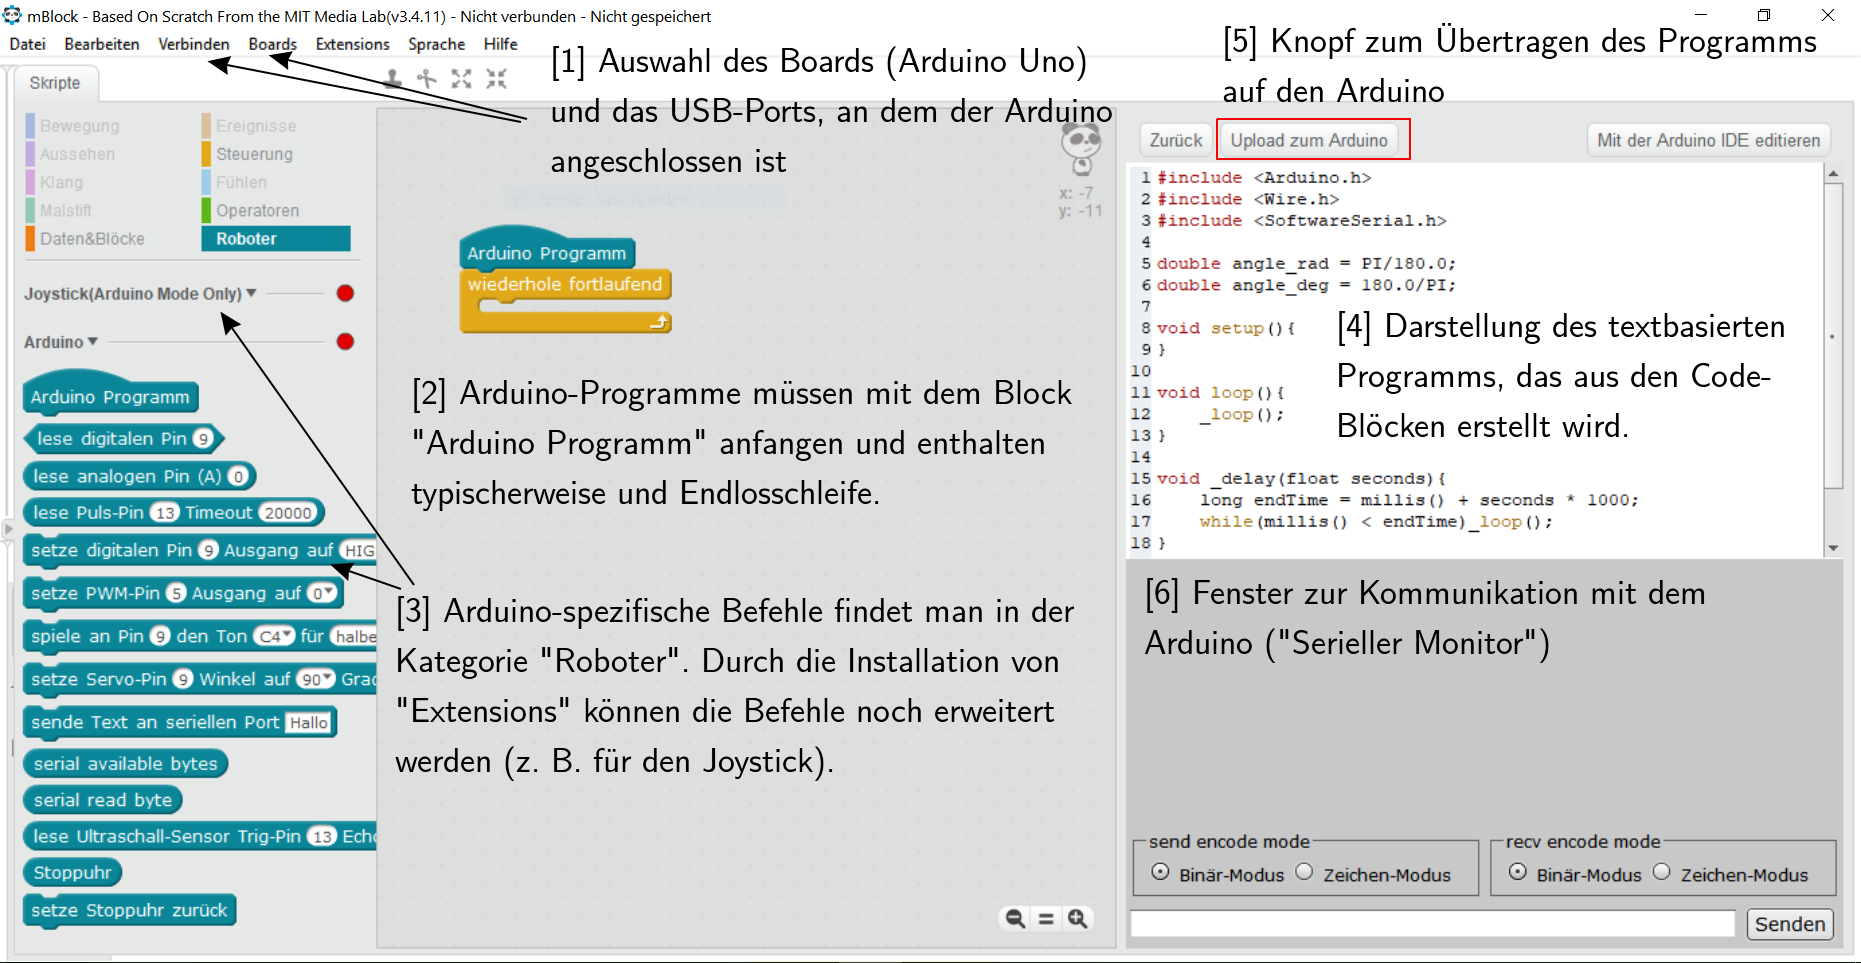
\includegraphics[width=1.2\textwidth]{pics/mblock-arduinomodus.PNG}
		\caption{Übersicht über die Programmierumgebung \emph{mBlock} im Arduino-Modus.}
		\label{abb:mblock-arduinomodus}
	\end{adjustwidth*}
\end{figure}

Die Programmierumgebung \emph{mBlock} wurde im Wesentlichen dafür erstellt, dass man die firmeneigenen Roboter namens \emph{mBot} programmieren kann. Diese basieren auf einem Arduino, der die angeschlossenen Motoren und Sensoren steuert und per \emph{mBlock} programmiert wird. Gleichzeitig ermöglicht es \emph{mBlock} auch, den Arduino als eigenständigen Mikrocontroller zu programmieren. Dies ist der Modus, den wir benutzen werden. Man erreicht diesen Arduino-Modus unter \button{Bearbeiten} $\rightarrow$ \button{Arduino-Modus}. 

Als erstes muss der USB-Port ausgewählt werden, an dem der Arduino angeschlossen ist (unter \button{Verbinden}) und danach muss der Arduino Uno als Board ausgewählt werden (unter \button{Boards}). Damit sind alle Einstellungen vorgenommen, um den Arduino Uno mit mBlock programmieren zu können.

\newpage
\section{Digitale Ausgänge steuern}

\begin{ziel}
	\textbf{Ziel:} Es soll das erste Testprogramm auf den Arduino übertragen werden, mit dem man üblicherweise überprüft, ob der Arduino (oder ein anderer Mikrocontroller) richtig funktioniert. Dazu soll die bordeigene LED zum Blinken gebracht werden:
	\begin{itemize}[itemsep=0ex]
		\item Stelle LED an.
		\item Warte eine Sekunde.
		\item Stelle LED aus.
		\item Warte eine Sekunde.
		\item Wiederhole fortlaufend.
	\end{itemize}
\end{ziel}

\emph{Hinweise:} 
\medskip

\begin{minipage}{0.7\textwidth}
	Arduino-Programme müssen immer mit dem entsprechenden Startblock für ein Arduino-Programm beginnen (siehe Abbildung rechts.)
\end{minipage}
\begin{minipage}[]{0.3\textwidth}
	\centering
	
\includegraphics[width=0.75\textwidth]{pics/Arduino_Start_Block.png}
	\label{abb:arduinostartblock}
\end{minipage}


\begin{wrapfigure}{r}{0.4\textwidth}
	\centering
	
\includegraphics[width=0.4\textwidth]{pics/digitalWriteBlock.png}
	\label{abb:digitalwriteblock}
\end{wrapfigure}
Die bordeigene LED ist mit dem (digitalen) Pin Nummer 13 verbunden und kann darüber gesteuert werden. Zur Steuerung von digitalen Pins nutzt man den rechts abgebildeten Block.

Mit dem Knopf \button{Upload zum Arduino} lässt sich das fertige Programm auf den Arduino übertragen. Wenn alles klappt, sollte nun die bordeigene LED blinken.

\begin{aufgabe}
	Wir nutzen in den ersten Kapiteln sehr häufig LEDs, weil sich die Grundlagen mit ihnen einfach erarbeiten lassen, aber auch weil sie eine enorme Bedeutung in der heutigen Welt haben. Notiere dir zur Verdeutlichung eine Woche lang alle Geräte, die dir begegnen oder die dir einfallen, in denen LEDs verbaut sind.
\end{aufgabe}


\newpage
\section{Aufbau von Schaltungen auf der Steckplatine}

In der Regel braucht man für interressante Geräte zusätzliche \emph{Hardware} (Sensoren, Motoren, \dots), die am Arduino angeschlossen wird. Bevor diese fest verlötet werden, nutzt man normalerweise Steckverbindungen bzw. baut die Schaltung auf einem kleinen Steckbrett auf, auf dem man die Verbindungen schnell wieder lösen kann, falls nötig. Steckbretter sind aus dem Physikunterricht bekannt. Abbildung \ref{abb:steckbrett} zeigt, welche Kontakte auf dem Steckbrett miteinander verbunden sind.

\begin{figure}[h]
	\centering
	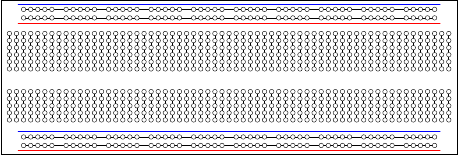
\includegraphics[width=0.8\textwidth]{./Zeichnungen/steckbrett.png}
	\caption{Die Steckverbindungen sind außen in Längsrichtung und innen in Querrichtung miteinander verbunden.}
	\label{abb:steckbrett}
\end{figure}

\begin{ziel}
	\textbf{Ziel:} Eine externe LED an Pin 13 soll zum Leuchten gebracht werden. Diese kann genutzt werden, um das Blinken einer Alarmanlagen-LED zu simulieren.
\end{ziel}

\emph{Hinweise:} 

Es kann das Programm aus dem vorherigen Abschnitt wieder verwendet werden. Allerdings gibt es ein Problem: Wenn der digitale Pin auf \texttt{HIGH} gesetzt wird, bedeutet das, dass er eine Spannung von 5V gegenüber GND ausgibt. Die LED verträgt jedoch nur (je nach Farbe) gut 2 V. Daher ist die LED mit einem Vorwiderstand von $\SI{330}{\SIUnitSymbolOhm}$ verbunden.

Die LED ist ein sogenanntes gepoltes Bauteil. Das heißt, dass einer der Kontaktstifte der LED an den Plus-Kontakt angeschlossen werden \emph{muss} und der andere an den Minus-Kontakt angeschlossen werden \emph{muss}.

%\bigskip
%\textbf{Projekt 1: Ampel}
\begin{projekt}[Ampel]\label{proj:ampel}
	Baue und programmiere eine Ampelschaltung!
	
	\emph{Für Schnelle:} Erweitere die Ampel um einen Nachtmodus.
\end{projekt}

%\bigskip
%\textbf{Projekt 2: Augentestgerät}

\begin{projekt}[Augentestgerät]\label{proj:augentest}
	Moderne Fernseher nutzen meist eine Bildwiederholungsrate von 144 Hertz; das bedeutet, es werden 144 Bilder pro Sekunde eingespielt. Finde mithilfe des Blink-Programms heraus, ab welchem Blinkintervall du kein Flackern mehr wahrnimmst und berechne, wie viele \enquote{Bilder} pro Sekunde sich daraus ergeben. Vergleiche diesen Wert mit der Bildwiederholungsrate im Fernsehen.
	
	{\scriptsize Idee: Frick, Fritsch und Trick (2015): \emph{Einführung in Mikrocontroller - Der Arduino als Steuerzentrale}, Bad Saulgau}
\end{projekt}


\newpage

\section{Widerstand, Spannung und elektrische Stromstärke berechnen}

\begin{wrapfigure}{r}{0.2\textwidth}
	\centering
	\vspace{-\baselineskip}
	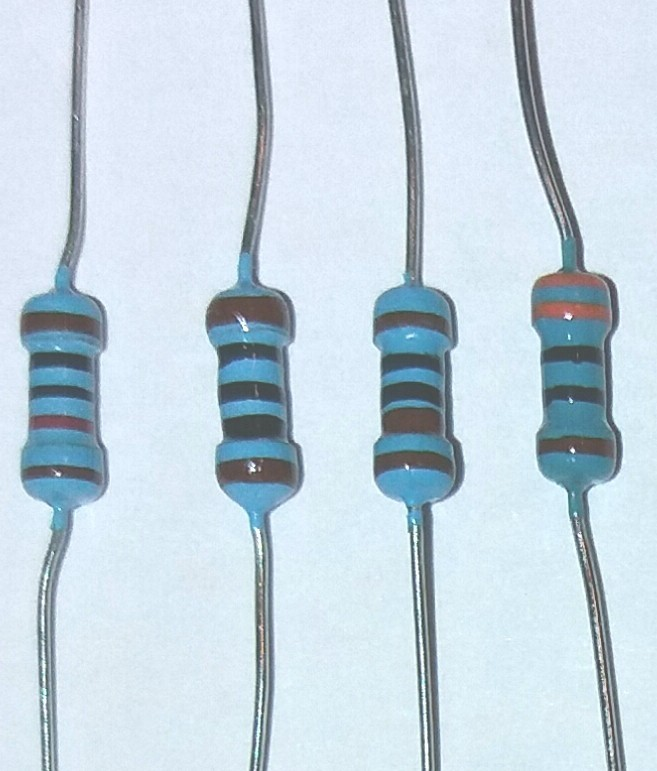
\includegraphics[width=0.18\textwidth,angle=90]{pics/Widerstaende.jpg}
	\vspace{-3\baselineskip}
	\label{abb:widerstaende}
\end{wrapfigure}
Im vorherigen Abschnitt war die Größe des Vorwiderstands mit $\SI{330}{\SIUnitSymbolOhm}$ vorgegeben. 
In unserem Bausatz finden sich jedoch viele weitere Widerstände, die teilweise größer und teilweise kleiner sind.

\textbf{Vorüberlegung:} Wird die LED heller oder dunkler leuchten, wenn man den Vorwiderstand vergrößert? Begründe deine Vermutung.

\begin{figure}[H]
	\centering
	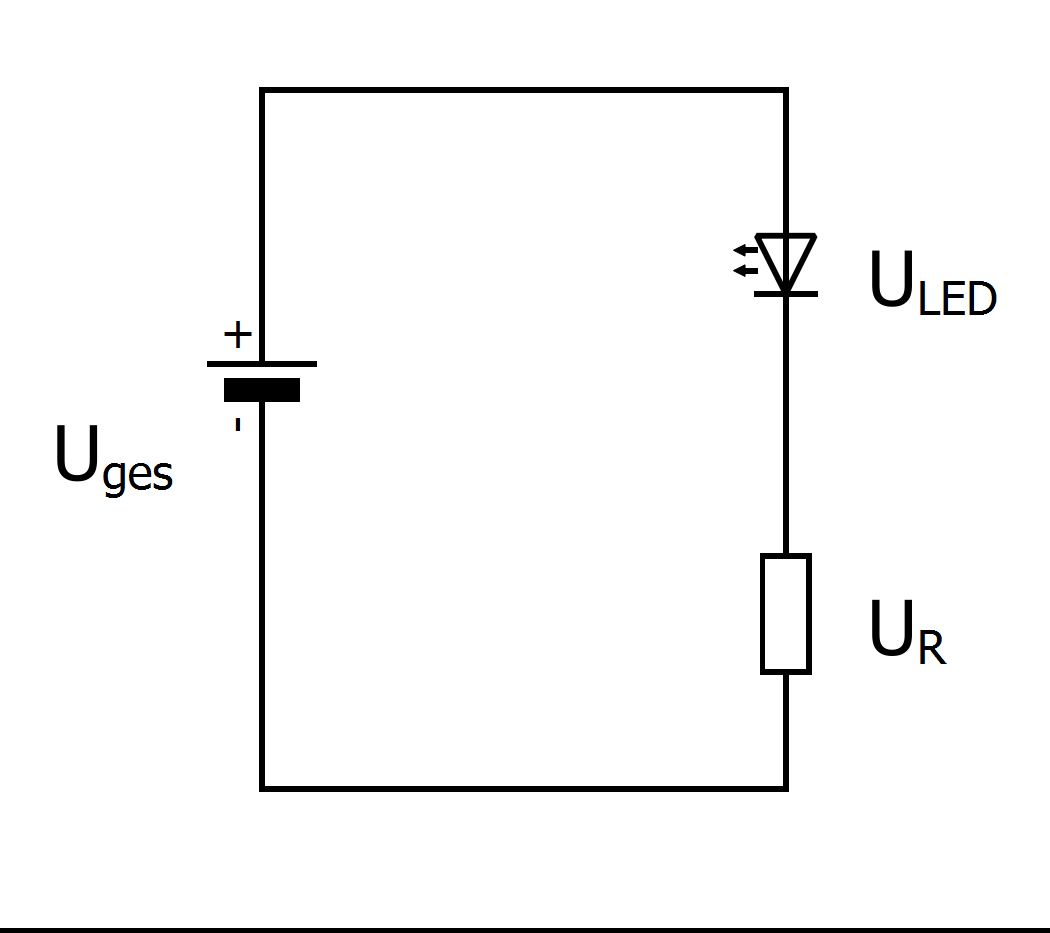
\includegraphics[width=0.35\textwidth]{./Zeichnungen/ReiheLEDWiderstand.png}
	\caption{Reihenschaltung von LED und Vorwiderstand an einer Spannungsquelle.}
	\label{abb:reiheledwiderstand}
\end{figure}
% Vorüberlegungen zur gleichzeitigen Wiederholung der Gesetze für die Reihenschaltung:
% Der Strom durch den Widerstand wird kleiner, wenn der Widerstand größer wird. Da die Stromstärke überall gleich groß ist, wird auch die Stromstärke in der LED kleiner.
% Die LED leuchtet, weil sie elektrische Energie in Lichtenergie umwandelt. Ein Maß für die elektrische Energie der Teilchen ist die Spannung. Wenn der Widerstand größer wird, wird auch die Spannung, die dort abfällt, größer (die Teilchen brauchen mehr Energie, um hindurch zu kommen). Daher wird die Spannung an der LED kleiner, denn die Gesamtspannung von 5V bleibt gleich und beide Spannungen addieren sich zur Gesamtspannung.
% Die Widerstände der Bauteile addieren sich ebenfalls zum Gesamtwiderstand.

Nach den Vorüberlegungen ist klar, dass ein größerer Widerstand für die LED kein Problem darstellt. Aber wie sieht es mit einem kleineren Widerstand aus? Der Widerstand muss schließlich in jedem Fall verhindern, dass die LED stärker belastet wird als sie aushält\dots

\begin{ziel}
	\textbf{Frage:} Wie groß muss der Vorwiderstand einer LED mindestens sein, damit sie nicht durchbrennt?
\end{ziel}

\emph{Hinweise:}
\begin{itemize}[itemsep=0mm,parsep=0mm]
	\item Wenn ein Digitalpin auf \texttt{HIGH} gesetzt wird, dann gibt er eine Spannung von 5V gegenüber GND aus.
	\item Durch eine LED darf höchstens ein Strom von $\SI{20}{\milli\ampere}$ fließen.
	\item Je nach Farbe halten LEDs eine andere maximale Spannung aus:
	
	\begin{tabular}{l|l|l|l}
		Farbe & rot & gelb/grün & blau/weiß \\ \hline
		$U_{LED}$ & 1,6\,V - 2,2\,V & 1,9\,V - 2,5\,V & 2,7\,V - 3,5\,V \\
	\end{tabular}
\end{itemize}

\begin{zsfg}{{Widerstand, Spannung und Stromstärke}}
	\begin{wrapfigure}{r}{0.15\textwidth}
		\vspace{-\baselineskip}
		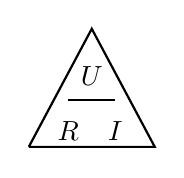
\begin{tikzpicture}
			\draw [black, thick] (0,0) -- (0.8,1.5) -- (1.6,0) -- (0,0);
			\node at (0.8,0.9) {\color{black}$U$};
			\draw [black, thick] (0.5,0.6) -- (1.1,0.6);
			\node at (0.5,0.2) {\color{black}$R$};
			\node at (1.1,0.2) {\color{black}$I$};
		\end{tikzpicture}
	\end{wrapfigure}
	Der Widerstand $R$ ist definiert als das Verhältnis von Spannung $U$ zu Stromstärke $I$:
	\begin{equation*}
		R=\frac{U}{I}.
	\end{equation*}
	
	Ein Widerstand heißt \emph{ohmscher Widerstand}, wenn das Verhältnis $\frac{U}{I}$ stets gleich groß ist (also wenn $R$ unabhängig von Stromstärke und Spannung konstant ist).
\end{zsfg}
\begin{tcolorbox}[equal height group=A,enhanced, colback=CadetBlue!70!green, coltext=black, colframe=DarkCyan!70!DarkGreen, width=0.48\textwidth, before=, after=\hfill, adjusted title={Elektrische Stromstärke und Spannung in der Reihenschaltung}, colbacktitle=CadetBlue!70!green, coltitle=black, fonttitle=\bfseries]
	\begin{figure}[H]
		\centering
		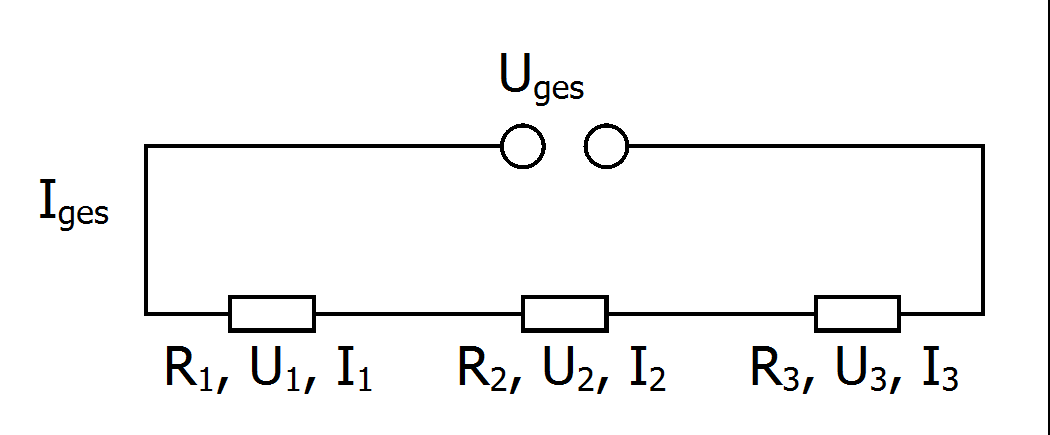
\includegraphics[width=\textwidth]{./Zeichnungen/reihenschaltung.png}
	\end{figure}
	\begin{itemize}[parsep=0ex,itemsep=0ex,leftmargin=*]
		\item In einer Reihenschaltung ist die Stromstärke an jeder Stelle gleich groß:
		\begin{equation*}
			I_{ges}=I_1=I_2= I_3=\dots
		\end{equation*}
		\item In einer Reihenschaltung teilt sich die Gesamtspannung auf die einzelnen Bauteile auf:
		\begin{equation*}
			U_{ges}=U_1 + U_2 + U_3+\dots
		\end{equation*}
		\item In einer Reihenschaltung addieren sich die Einzelwiderstände zum Gesamtwiderstand:
		\begin{equation*}
			R_{ges}=R_1+R_2+R_3+\dots
		\end{equation*}
	\end{itemize}
\end{tcolorbox}
\begin{tcolorbox}[equal height group=A,enhanced, colback=CadetBlue!70!green, coltext=black, colframe=DarkCyan!70!DarkGreen, width=0.48\textwidth, before=, after=\hfill, adjusted title={Elektrische Stromstärke und Spannung in der Parallelschaltung}, colbacktitle=CadetBlue!70!green, coltitle=black,fonttitle=\bfseries]
	\begin{figure}[H]
		\centering
		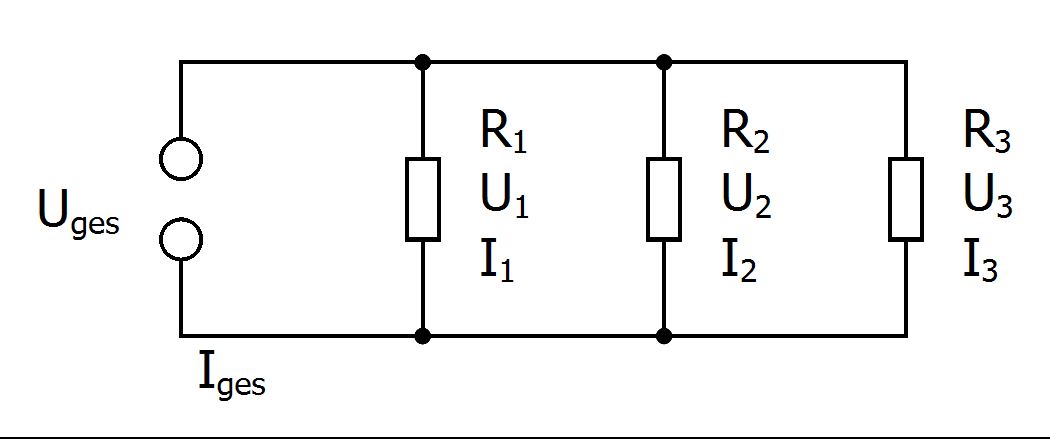
\includegraphics[width=\textwidth]{./Zeichnungen/parallelschaltung.png}
	\end{figure}
	\begin{itemize}[parsep=0ex,itemsep=0ex,leftmargin=*]
		\item In einer Parallelschaltung teilt sich die Gesamtstromstärke auf die einzelnen Zweige auf:
		\begin{equation*}
			I_{ges}=I_1+I_2+ I_3+\dots
		\end{equation*}
		\item In einer Parallelschaltung ist die Spannung in jedem Zweig gleich groß:
		\begin{equation*}
			U_{ges}=U_1=U_2=U_3=\dots
		\end{equation*}
		\item In einer Parallelschaltung ist der Kehrwert des Gesamtwiderstands gleich der Summe der Kehrwerte der einzelnen Widerstände:
		\begin{equation*}
			\frac{1}{R_{ges}} = \frac{1}{R_1} + \frac{1}{R_2} + \frac{1}{R_3} + \dots
		\end{equation*}
	\end{itemize}
\end{tcolorbox}

\begin{aufgabe}
	In unserem Starter Kit ist ein 9V Akku untergebracht. Berechne den mindestens notwendigen Vorwiderstand, wenn eine
	rote LED an den 9V Block angeschlossen wird.
\end{aufgabe}

\begin{aufgabe}
	\smallbreak
	\textbf{a)} An einem 9V Block sollen drei rote LEDs in Reihe geschaltet betrieben werden. Zeichne einen Schaltplan und berechne den passenden Vorwiderstand.
	
	\textbf{b)} An einem 9V Block sollen drei rote LEDs parallel geschaltet betrieben werden. Zeichne einen Schaltplan und berechne den passenden Vorwiderstand.
\end{aufgabe}
\vfill

\newpage
\begin{projekt}[Farbenspektakel mit RGB-LED]\label{proj:rgbled1}
	
	\smallskip
	\begin{minipage}{0.45\textwidth}
		Mit einer RGB-LED können die verschiedensten Farben erzeugt werden, die zum Beispiel in Smartphones als Status-LED genutzt werden. RGB steht für Rot, Grün und Blau. In einer RGB-LED sind also drei LEDs gleichzeitig verbaut, die sich in unserem Fall eine gemeinsame Anode (Kontakt mit GND) teilen. Die Anode gehört zum längsten Beinchen.
	\end{minipage}
	\hfill
	\begin{minipage}{0.5\textwidth}
		\begin{figure}[H]
			\hfill
			\begin{minipage}{0.48\textwidth}
				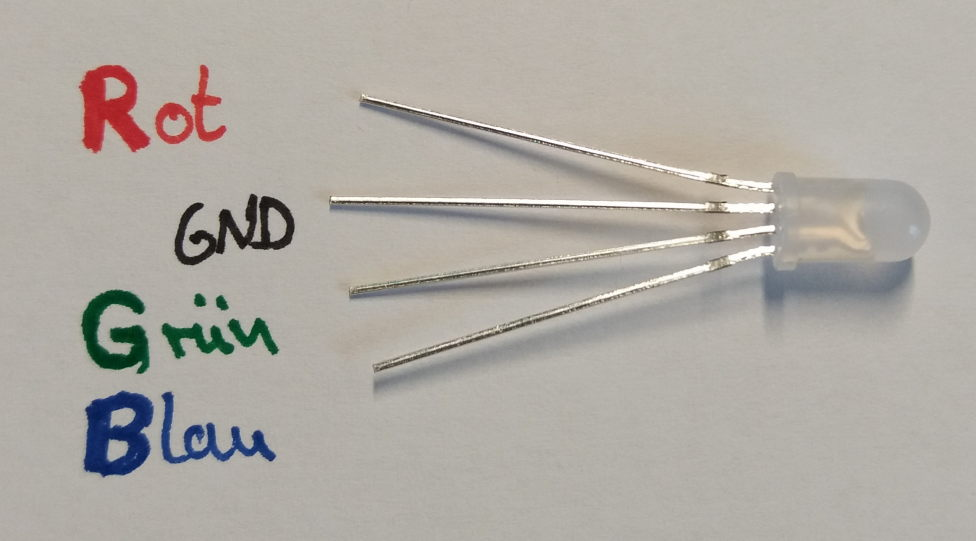
\includegraphics[width=\textwidth]{pics/rgb-led.jpg}
				\caption{RGB-LED}
			\end{minipage}
			\hfill
			\begin{minipage}{0.48\textwidth}
				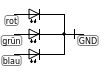
\includegraphics[width=\textwidth]{pics/rgb-led-schaltplan.png}
				\caption{Verschaltung der RGB-LED.}
			\end{minipage}
			\hfill
			\label{abb:rgb-led}
		\end{figure}
	\end{minipage}
	\bigskip
	
	\begin{wrapfigure}{r}{0.25\textwidth}
		\centering
		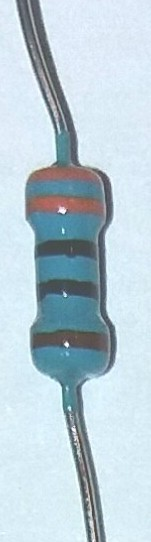
\includegraphics[angle=90,width=0.2\textwidth]{pics/330ohm.jpg}
	\end{wrapfigure}
	Schließe die RGB-LED an den Arduino an. \emph{Achte darauf, dass zwischen den Plus-Kontakten der LEDs und den digitalen Pins ein Widerstand von von $\SI{330}{\ohm}$ geschaltet ist.} Der Widerstand lässt sich an der Reihenfolge der Ringe erkennen: Orange - Orange - Schwarz - Schwarz - Braun.
	
	\medbreak
	\textbf{a)} Experimentiere mit den verschiedenen Farben. Notiere dir alle möglichen Farbtöne und wie diese zusammengesetzt sind.
		
	\medskip
	\textbf{b)} \emph{Zur Reflexion der Berechnung des Vorwiderstands:} Begründe, warum der unten berechnete Vorwiderstand zu niedrig ist. Erkläre, wie man stattdessen vorgehen müsste und gib den korrekten Wert für einen möglichen gemeinsamen Vorwiderstand an.
\end{projekt}
\marginpar{%
	\parbox{1.5cm}{%
		\footnotesize%
		Wie man weitere Farben erzeugt, erfährst du in \ref{proj:rgbled2}.
	}
}

\vspace{2\baselineskip}
\begin{tcolorbox}[sharp corners]
	\begin{wrapfigure}{r}{0.4\textwidth}
		\centering
		\vspace{-\baselineskip}
		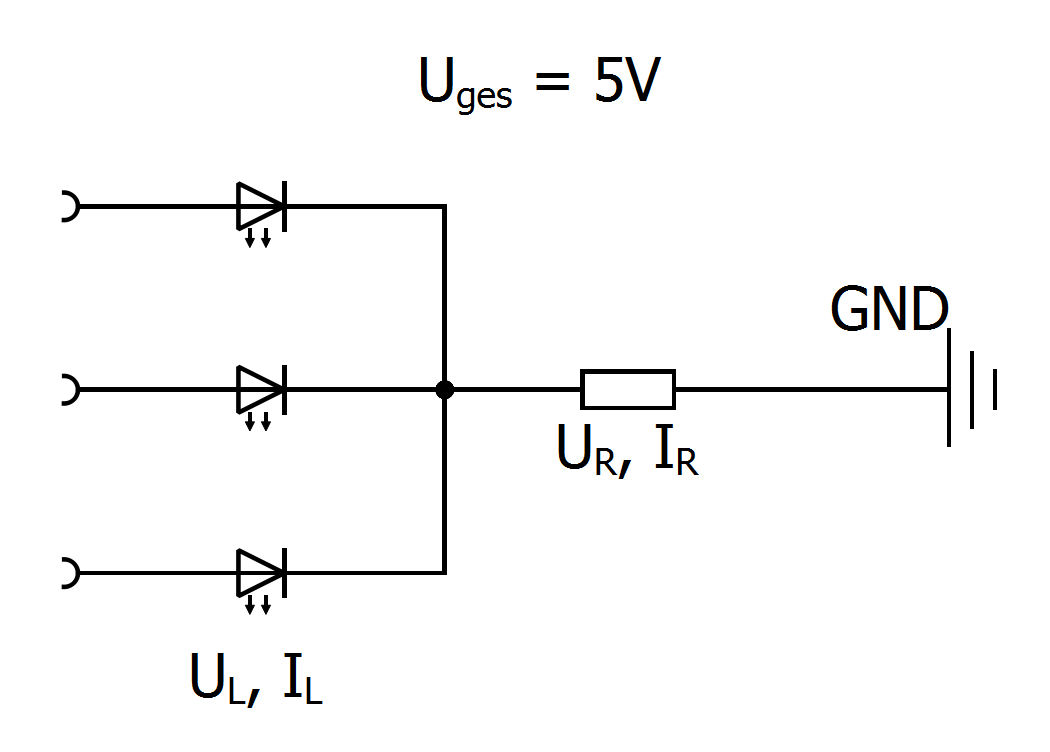
\includegraphics[width=0.4\textwidth]{./Zeichnungen/schaltplan-rgb-led-berechnung.png}
	\end{wrapfigure}
	$I_L = \SI{20}{\milli\ampere} = \SI{0,02}{\ampere} \quad \Longrightarrow \quad I_R = \SI{0,06}{\milli\ampere}$
	
	$U_L = \SI{2,2}{\volt}$ \quad (max. Spannung, die rote LEDs aushalten)
	
	$U_R = \SI{5}{\volt} - \SI{2,2}{\volt} = \SI{2,8}{\volt}$
	
	\begin{equation*}
		R = \frac{U_R}{I_R} = \frac{\SI{2,8}{\volt}}{\SI{0,06}{\ampere}} \approx \SI{46,67}{\ohm}
	\end{equation*}
	
	\bigskip
	Der Vorwiderstand sollte eine Größe von mindestens $\SI{50}{\ohm}$ haben.
\end{tcolorbox}

%Das Problem ist, dass auch nur eine LED angeschaltet sein kann und dann darf der Gesamtwiderstand nur 0,02 A durchlassen, muss also größer sein.

\newpage
\section{Widerstandsringe ablesen}

Leider sind die Widerstände zu klein, um ihren Wert darauf gut lesbar zu drucken. Daher werden die Widerstände mit Ringen versehen, aus deren Farbe sich die Größe des Widerstands ablesen lässt. Um den für die 7-Segment-Anzeige passenden Widerstand aus dem Bausatz auszuwählen, müssen wir diesen Farbcode lesen können.

Bei den blauen Kohleschichtwiderständen, die wir verwenden, gibt es fünf Ringe und jede Ringfarbe steht für eine Zahl. Die ersten drei Ringe bilden die ersten drei Ziffern des Widerstandswertes ab. Die darauf folgende Ringfarbe steht für die Zehnerpotenz, die mit den drei Ziffern multipliziert werden muss. Dies dient dazu, auch größere Widerstandswerte codieren zu können. Der letzte Ring wiederum soll einen etwas größeren Abstand haben und steht für die Fehlertoleranz des Widerstandswertes. In der Praxis lässt sich allerdings nicht immer gut erkennen, welcher Ring der letzte und welcher der erste ist\dots

\begin{figure}[H]
	\centering
	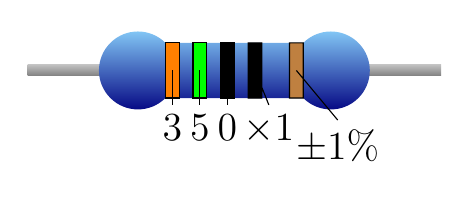
\begin{tikzpicture}[scale=0.35]
	\shade [top color=lightgray, bottom color=gray] (-5,0.8) rectangle (10,1.2);
	\shade [top color=LightSkyBlue, bottom color=NavyBlue] (0,0) -- (5,0) arc [start angle=-135, end angle=135, radius=1.414] -- (0,2) arc [start angle=45, end angle=315, radius=1.414];
	\draw [fill=orange] (0,0) rectangle ++(0.5,2) ++(-0.25,-1) -- ++(0,-1.25) [anchor =north] node {\Large 3};
	\draw [fill=green] (1,0) rectangle ++(0.5,2) ++(-0.25,-1) -- ++(0,-1.25) [anchor =north] node {\Large 5};
	\draw [fill=black] (2,0) rectangle ++(0.5,2) ++(-0.25,-1) -- ++(0,-1.25) [anchor =north] node {\Large 0};
	\draw [fill=black] (3,0) rectangle ++(0.5,2) ++(-0.25,-1) -- ++(0.5,-1.25) [anchor =north] node {\Large $\times 1$};
	\draw [fill=brown] (4.5,0) rectangle ++(0.5,2) ++(-0.25,-1) -- ++(1.5,-1.8) [anchor =north] node {\Large $\pm1\%$};
	\end{tikzpicture}
\end{figure}
Ein Beispiel: Die Ringfarben lauten orange - grün - schwarz - schwarz - braun. Anhand der folgenden Tabelle lässt sich daraus der Wert konstruieren: $3 - 5 - 0 - \cdot 1 (=10^0) - \pm 1\% $, kurz: $\SI{350}{\SIUnitSymbolOhm}\pm\SI{3,5}{\SIUnitSymbolOhm}$.

\begin{table}[H]
   \centering
   %\rowcolors{1}{lightgray}{white}
   \begin{minipage}[c]{\textwidth}
      \begin{tabu} to \textwidth {X[L,2]X[C]X[C]X[C]X[C,3]X[C,2]}
         \toprule
         \textbf{Ringfarbe} & \textbf{1. Ring} & \textbf{2. Ring} & \textbf{3. Ring} & \textbf{4. Ring (Multiplikator)} & \textbf{5. Ring (Toleranz)} \\
         \midrule
         \textcolor{black}{\rule{1cm}{0.4cm}} Schwarz & 0 & 0  & 0 & $\times 1$ / $\times 10^0$ & - \\
         \textcolor{brown}{\rule{1cm}{0.4cm}} Braun   & 1 & 1 & 1& $\times10$ / $\times 10^1$ & 1\% \\
         \textcolor{red}{\rule{1cm}{0.4cm}} Rot  & 2 & 2 & 2& $\times100$ / $\times 10^2$ & 2\% \\
         \textcolor{orange}{\rule{1cm}{0.4cm}} Orange & 3 & 3 & 3& $\times 1000$ / $\times 10^3$ & - \\
         \textcolor{yellow}{\rule{1cm}{0.4cm}} Gelb & 4 & 4 & 4& $\times 10.000$ / $\times 10^4$ & - \\
         \textcolor{green}{\rule{1cm}{0.4cm}} Grün  & 5 & 5 & 5& $\times 100.000$ / $\times 10^5$ & - \\
         \textcolor{blue}{\rule{1cm}{0.4cm}} Blau  & 6 & 6 & 6& $\times 1.000.000$ / $\times 10^6$ & - \\
         \textcolor{violet}{\rule{1cm}{0.4cm}} Lila & 7 & 7 & 7& - & - \\
         \textcolor{gray}{\rule{1cm}{0.4cm}} Grau   & 8 & 8 & 8& - & - \\
         \tikz \draw (0,0) rectangle (1,0.4); Weiß & 9 & 9 & 9& - & - \\
         \textcolor{Gold}{\rule{1cm}{0.4cm}} Gold & - & - & -& $\times 0.1$ / $\times 10^{-1}$ & 5\% \\
         \textcolor{lightgray}{\rule{1cm}{0.4cm}} Silber & - & - & -& $\times 0.01$ / $\times 10^{-2}$ & 10\% \\
         \bottomrule
      \end{tabu}
   \end{minipage}
   \caption{Tabelle zur Codierung der Widerstandswerte durch Farbringe.}
   \label{tab:farbcodierung}
\end{table}

\begin{aufgabe}
	Gib die Farbcodierung für einen Widerstand mit den folgenden Werten an:
	\begin{multicols}{2}
		\begin{enumerate}[label=\alph*),itemsep=0ex]
			\item $\SI{435}{\SIUnitSymbolOhm} (\pm 2\%)$,
			\item $\SI{570}{\kilo\SIUnitSymbolOhm} (\pm 5\%)$.
		\end{enumerate}
	\end{multicols}
\end{aufgabe}

\vfill
\newpage
\begin{aufgabe}
	
	\begin{minipage}{0.78\textwidth}
		\textbf{a)} Die rechte Abbildung zeigt die vier wichtigsten Widerstände, mit denen wir zu tun haben werden. Bestimme die jeweilige Größe der Widerstände.
		
		\textbf{b)} Thorsten hat die Ringe eines Widerstands abgelesen: Silber - rot - lila - lila - grün. Bestimme die Größe des Widerstands.
	\end{minipage}
	\hfill
	\begin{minipage}{0.2\textwidth}
		\begin{figure}[H]
			\centering
	%		\vspace{-\baselineskip}
			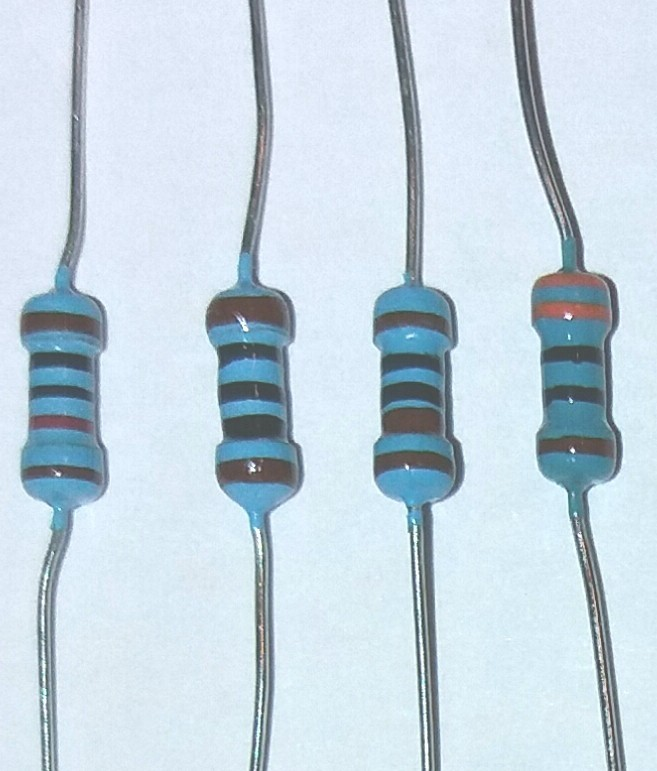
\includegraphics[width=0.8\textwidth,angle=90]{pics/Widerstaende.jpg}
			\label{abb:widerstaende2}
		\end{figure}
	\end{minipage}
	
	\medskip
	\emph{Zur Kontrolle:} \url{https://www.elektronik-kompendium.de/sites/bau/1109051.htm}
\end{aufgabe}


\subsection{Einfache Verwendung einer 7-Segment-Anzeige}

\begin{minipage}{0.58\textwidth}
	Unsere 7-Segment-Anzeige besteht aus sieben roten LEDs, die so angeordnet sind, dass sich mit ihnen eine Zahl darstellen lässt. Zusätzlich gibt es  zur leichteren Unterscheidung von 6 und 9 eine LED für den Punkt. \emph{Jede LED lässt sich einzeln über einen der Pins ansteuern, wobei sich alle LEDs einen gemeinsamen GND-Anschluss teilen.} Der zweite GND-Anschluss soll hier nicht genutzt werden, um die Schaltung so einfach wie möglich zu halten. Es wäre sehr umständlich, für jede LED einen eigenen Vorwiderstand anzuschließen; praktischer ist es, einen einzigen Vorwiderstand zwischen GND-Anschluss der 7-Segment-Anzeige und GND-Anschluss des Arduino anzubringen.
\end{minipage}
\hfill
\begin{minipage}{0.4\textwidth}
	\begin{figure}[H]
		\hfill
		\begin{minipage}{0.48\textwidth}
			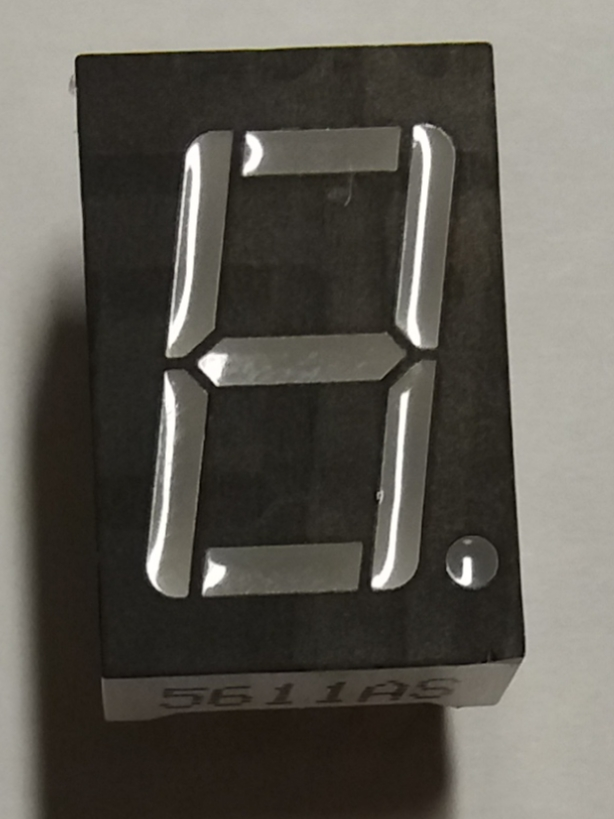
\includegraphics[width=\textwidth]{pics/7segmentanzeige-bild2.jpg}
			\caption{7-Segment-Anzeige}
			\label{abb:7segment-bild}
		\end{minipage}
		\hfill
		\begin{minipage}{0.48\textwidth}
			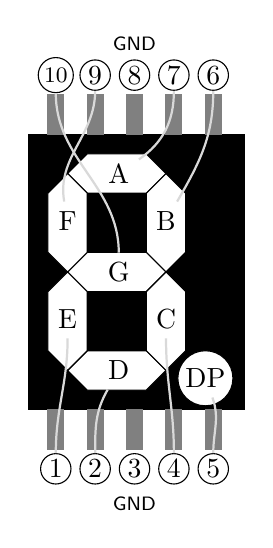
\begin{tikzpicture}[scale=0.5]
	% Rahmen der Anzeige
	\draw [fill=black] (0,0) rectangle (5.5,7);
	% Segment D
	\draw [fill = white] (1,1) -- ++(0.5,-0.5) -- ++ (1.5,0) -- ++ (0.5,0.5) -- ++ (-0.5,0.5) -- ++ (-1.5,0) -- ++(-0.5,-0.5)  node at ++(1.3,0) (segD) {D}; 
	% Segment G
	\draw [fill = white] (1,3.5) -- ++(0.5,-0.5) -- ++ (1.5,0) -- ++ (0.5,0.5) -- ++ (-0.5,0.5) -- ++ (-1.5,0) -- ++(-0.5,-0.5)  node at ++(1.3,0) (segG) {G};
	% Segment A
	\draw [fill = white] (1,6) -- ++(0.5,-0.5) -- ++ (1.5,0) -- ++ (0.5,0.5) -- ++ (-0.5,0.5) -- ++ (-1.5,0) -- ++(-0.5,-0.5)  node at ++(1.3,0) (segA) {A};
	% Segment E
	\draw [fill = white] (1,1) -- ++ (0.5,0.5) -- ++ (0,1.5) -- ++ (-0.5,0.5) -- ++ (-0.5,-0.5) -- ++ (0,-1.5) -- ++ (0.5,-0.5) node at ++ (0,1.3) (segE) {E};  
	% Segment C
	\draw [fill = white] (3.5,1) -- ++ (0.5,0.5) -- ++ (0,1.5) -- ++ (-0.5,0.5) -- ++ (-0.5,-0.5) -- ++ (0,-1.5) -- ++ (0.5,-0.5) node at ++ (0,1.3) (segC) {C};
	% Segment F
	\draw [fill = white] (1,3.5) -- ++ (0.5,0.5) -- ++ (0,1.5) -- ++ (-0.5,0.5) -- ++ (-0.5,-0.5) -- ++ (0,-1.5) -- ++ (0.5,-0.5) node at ++ (0,1.3) (segF) {F};
	% Segment B
	\draw [fill = white] (3.5,3.5) -- ++ (0.5,0.5) -- ++ (0,1.5) -- ++ (-0.5,0.5) -- ++ (-0.5,-0.5) -- ++ (0,-1.5) -- ++ (0.5,-0.5) node at ++ (0,1.3) (segB) {B};
	% Punkt DP
	\draw [fill = white] (4.5,0.8) circle [radius=0.7cm] node (segDP) {DP};
	% Kontaktstifte
	\foreach \x in {0.5, 1.5, ..., 4.5} {
		\draw [draw=gray, fill=gray] (\x,0) rectangle ++(0.4,-1);
		\draw [draw=gray, fill=gray] (\x,7) rectangle ++(0.4,1);
	}
	% Nummerierung der Kontaktstifte
	\node at (1-0.3,-1.5) [circle, draw, inner sep=1pt] (pin1) {1};
	\node at (2-0.3,-1.5) [circle, draw, inner sep=1pt] (pin2) {2};
	\node at (3-0.3,-1.5) [circle, draw, inner sep=1pt] (pin3) {3};
	\node at (4-0.3,-1.5) [circle, draw, inner sep=1pt] (pin4) {4};
	\node at (5-0.3,-1.5) [circle, draw, inner sep=1pt] (pin5) {5};
	%	\foreach \x in {9,...,6}{
	%		\node at (11-\x-0.3,8.5) [circle, draw, inner sep=1pt] {\x};
	%	}
	\node at (1-0.3,8.5) [circle, draw, inner sep=1pt] (pin10) {\footnotesize 10};
	\node at (11-9-0.3,8.5) [circle, draw, inner sep=1pt] (pin9) {9};
	\node at (11-8-0.3,8.5) [circle, draw, inner sep=1pt] (pin8) {8};
	\node at (11-7-0.3,8.5) [circle, draw, inner sep=1pt] (pin7) {7};
	\node at (11-6-0.3,8.5) [circle, draw, inner sep=1pt] (pin6) {6};
	\node at (2.7,-2.4) {\scriptsize\sffamily GND};
	\node at (2.7,9.3) {\scriptsize\sffamily GND};
	% Verbindungen
	\draw [gray!30!white, thick] (segA) to [out=35,in=270] (pin7); %out= Winkel beim Verlassen, in = Winkel beim Eintreffen
	\draw [gray!30!white, thick] (segB) to [out=60,in=270] (pin6);
	\draw [gray!30!white, thick] (segC) to [out=-90,in=90] (pin4);
	\draw [gray!30!white, thick] (segD) to [out=-120,in=90] (pin2);
	\draw [gray!30!white, thick] (segE) to [out=-90,in=90] (pin1);
	\draw [gray!30!white, thick] (segF) to [out=100,in=270] (pin9);
	\draw [gray!30!white, thick] (segG) to [out=90,in=270] (pin10);
	\draw [gray!30!white, thick] (segDP) to [out=-70,in=90] (pin5);
\end{tikzpicture}
			\caption{Pin-Diagramm der 7-Segment-Anzeige.}
			\label{abb:7segment-pins}
		\end{minipage}
		\hfill
	\end{figure}
\end{minipage}

\begin{aufgabe}
	\begin{enumerate}[label=\alph*), itemsep=0ex,parsep=0mm]
		\item Zeichne einen vereinfachten Schaltplan der 7-Segment-Anzeige, %
		\marginpar{%
			\textattachfile[description={Druckvorlage zu Kap. \thechapter, Schaltplan mit Arduino}]{./Zeichnungen/Schaltplan-Arduino-Vorlage.pdf}{
			\footnotesize%
			\drucker Vorlage%
			}%
			%\href{run:./Zeichnungen/Schaltplan-Arduino-Vorlage.pdf}{Vorlage}% ./ verweist auf das aktuelle Verzeichnis; ../ auf das übergeordnete
			\footnotesize%
			\\öffnen%
		}
		in dem die LEDs einzeln eingezeichnet sind.
		\item Als gemeinsamen Vorwiderstand der acht LEDs (Anzeige \& Punkt) nutzen wir einen $\SI{330}{\ohm}$-Widerstand. Berechne die Gesamtstromstärke und die Stromstärke in jeder LED bei Darstellung einer 1 und einer 8 (jeweils ohne Punkt).
	\end{enumerate}
\end{aufgabe}

\begin{projekt}[Raketencountdown]\label{proj:raketencountdown}
	Suche dir nun einen passenden Widerstand für die 7-Segment-Anzeige heraus und verbinde beide mit dem Arduino. Programmiere dann einen Raketencountdown, der von 9 rückwärts bis 0 zählt.
	
	\emph{Tipp:} Erstelle dir zuerst eine Tabelle, in der du übersichtlich festhälst, welche LEDs für welche Zahl an sein müssen und mit welchen Pins am Arduino diese verbunden sind.
	
	\emph{Für Schnelle:} Man kann mit einer 7-Segment-Anzeige auch Buchstaben darstellen und nacheinander durchlaufen lassen!
	
	{\scriptsize Idee: Frick, Fritsch und Trick (2015): \emph{Einführung in Mikrocontroller - Der Arduino als Steuerzentrale}, Bad Saulgau}
\end{projekt}

%Beurteile anhand des unten abgebildeten Informationskastens, ob man die 7-Segment-Anzeige gefahrlos mit nur einem Vorwiderstand an den Arduino anschließen darf.
%\begin{zsfg}{Kennwerte zur maximalen Stromausgabe und Stromaufnahme}
%	
%	Wenn die angegebenen Maximalwerte überschritten werden, wird der Arduino Schaden nehmen!
%	\begin{itemize}[itemsep=0ex]
%		\item Max. Stromausgabe an Digitalpins: $\SI{40}{\milli\ampere}$ (empfohlen: $\SI{20}{\milli\ampere}$)
%		\item Max. Stromausgabe am VCC-Pin: $\SI{200}{\milli\ampere}$
%		\item Max. Stromaufnahme am GND-Pin: $\SI{200}{\milli\ampere}$
%	\end{itemize}
%\end{zsfg}
%\begin{flushright}
%	\vspace{-\baselineskip}
%	\footnotesize
%	Quelle: \url{https://playground.arduino.cc/Main/ArduinoPinCurrentLimitations}
%\end{flushright}

%\begin{minipage}{0.65\textwidth}
\vfill
\newpage
\section{Das elektrische Potential an digitalen Eingängen}

In diesem Abschnitt soll geklärt werden, wie man dem Arduino beibringt, auf bestimmte Eingaben aus der Umwelt zu reagieren. Konkret soll am Ende eine Fußgängerampel und eine Juke-Box gebaut werden, die auf Knopfdruck reagieren. Um verstehen zu können, wie der Arduino Signale aus der Umwelt registriert, muss jedoch zuerst geklärt werden, was sich hinter dem \emph{elektrischen Potential} verbirgt. Dazu machen wir einen kleinen Exkurs\dots

\subsection{Eine Analogie für das elektrische Potential}

\marginpar{%
	\textattachfile[description={Folie zu Kap. \thechapter, El. Potential}]{./Auftraege/kap3-auftrag-potential.pdf}{%
	\footnotesize\folie Folie%
	}%
	\footnotesize%
%	\folie \href{run:./Auftraege/kap3-auftrag-potential.pdf}{Folie}%
	\\öffnen
}
\begin{ziel}
	\textbf{a)} Anna und Bert schauen auf dasselbe Fenster. %
	Anna meint, das Fenster befinde sich in 1 Meter Höhe. Bert hingegen meint, das Fenster befinde sich in 4 Meter Höhe. Beide haben jeweils für sich betrachtet Recht. Wie kann das sein?
	
	\textbf{b)} Die Vase fällt einen Meter tief. Gib an, wie\dots
	\begin{itemize}[itemsep=0ex]
		\item \dots Anna die Höhenenergie nach dem Fallen berechnet und wie sie die Höhenenergie berechnet, die in Bewegungsenergie umgewandelt wurde.
		\item \dots Bert die Höhenenergie nach dem Fallen berechnet und wie er die Höhenenergie berechnet, die in Bewegungsenergie umgewandelt wurde.
	\end{itemize}

	Hinweis: $E_H=m\cdot g\cdot h$
\end{ziel}

Bei der Berechnung der Höhenenergie muss stets festgelegt werden, wo das \emph{Nullniveau} ist; das bedeutet: Wo die Höhe gemessen wird. Damit wird festgelegt: Bei dieser Grundhöhe ist die Höhenenergie null. Wenn nun eine Vase von der Fensterbank auf den Boden im Raum von Anna fällt, dann hat sie etwas Höhenenergie in Bewegungsenergie umgewandelt - und zwar genau die Höhenenergie, die einem Meter Höhendifferenz entspricht, denn sie ist einen Meter tief gefallen. \emph{Diese Differenz in der Höhe und der Höhenenergie ist unabhängig davon, welche Grundhöhe man betrachtet.} Sowohl aus Annas als auch aus Berts Sicht ist die Vase einen Meter tief gefallen.

\begin{zsfg}{Elektrisches Potential}
	So wie die Höhendifferenz ein Maß für die Höhenenergie ist, die umgewandelt wird (z. B. in Bewegungsenergie), ist die Spannung ein Maß für die elektrische Energie, die an einer LED, einem Widerstand etc. umgewandelt wird. Das elektrische Potential hingegen ist wie die Höhe ein Maß für die elektrische Energie der Elektronen im Stromkreislauf. Es kann nur in Bezug auf ein Nullniveau (\enquote{Ground}/GND) angegeben werden. Die Einheit des elektrischen Potentials ist Volt.
	
	Elektrisches Potential am GND-Pin: 0V
	
	Elektrisches Potential am 5V-Pin: 5V
\end{zsfg}

\newpage

\begin{aufgabe}
	
	\textbf{a)} Vervollständige die folgende Tabelle von Analogien.
	\begin{table}[H]
		\centering
		\begin{minipage}[c]{\textwidth}
			\begin{tabu} to \textwidth {X[C]|X[C]}
				\toprule
				\textbf{Mechanik} & \textbf{Elektrik} \\
				\toprule
				Höhenenergie \bigskip &  \\
				\midrule
				& Elektrisches Potential \bigskip \\
				\midrule
				Höhendifferenz \bigskip &  \\
				\midrule
				Grundhöhe \bigskip&  \\
				\bottomrule
			\end{tabu}
		\end{minipage}
		%   \caption{}
		\label{tab:analogie-potential}
	\end{table}
	
	\textbf{b)} Erkläre, welche der oben genannten Größen in der Mechanik bzw. der Elektrik abhängig von der Festlegung eines Nullniveaus sind.
\end{aufgabe}

\newpage
\subsection{Verwendung eines Tasters}
\label{sec:taster}

\begin{ziel}
	\textbf{Ziel:} Mithilfe des Arduino soll der Zustand eines Tasters eingelesen werden, um damit eine Fußgängerampel zu bauen.
\end{ziel}

\begin{wrapfigure}{r}{0.25\textwidth}
	\centering
	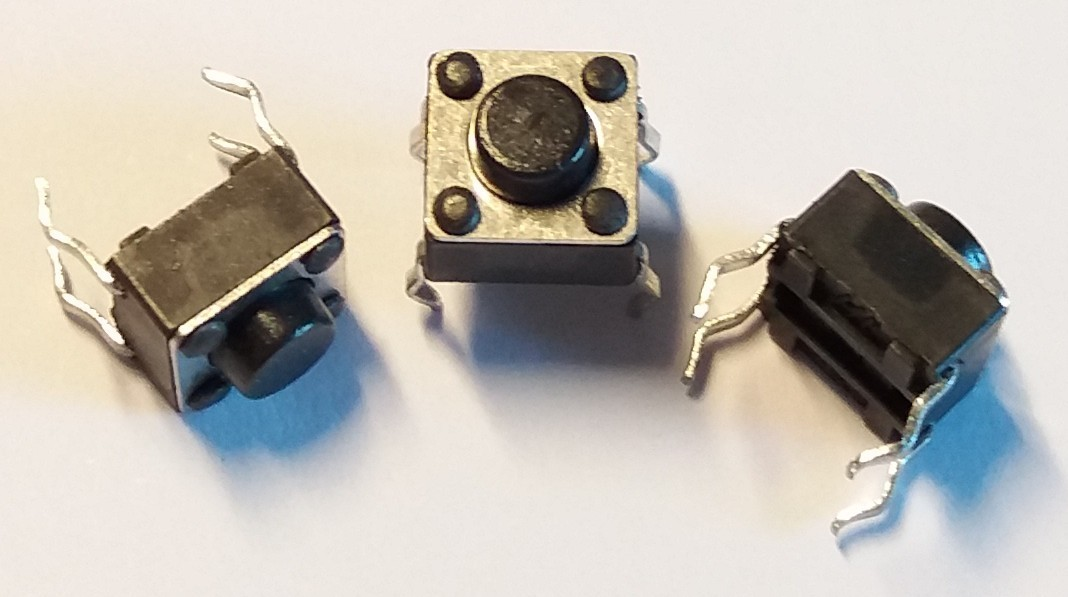
\includegraphics[width=0.25\textwidth]{pics/taster.jpg}
	\caption{Drei Taster.}
\end{wrapfigure}
Ein Taster ist wie ein Schalter, kann also geschlossen sein (Strom fließt) oder offen sein (Strom fließt nicht). Im Gegensatz zum Schalter springt ein Taster aber automatisch wieder in den offenen Zustand zurück, wenn er losgelassen wird.
 
In der unten abgebildeten Schaltplan ist dargestellt, wie man einen Taster am Arduino so anschließt, dass man seinen Zustand im digitalen Pin 3 auslesen kann.

\begin{aufgabe}\emph{Pulldown-Widerstand}
	
	Markiere die Kabel farbig, sodass die Kabel, die auf dem gleichen elektrischen Potential liegen, die gleiche Farbe haben. Notiere zudem den Wert des elektrischen Potentials.
\end{aufgabe}
\marginpar{%
	\textattachfile[description={Druckvorlage zu Kap. \thechapter, El. Potential an Tastern}]{./Auftraege/kap3-druckvorlage-taster.pdf}{
	\footnotesize%
	\drucker Vorlage%
	}%
	%\href{run:./Auftraege/kap3-druckvorlage-taster.pdf}{Vorlage}% ./ verweist auf das aktuelle Verzeichnis; ../ auf das übergeordnete
	\footnotesize%
	\\öffnen%
}

\begin{figure}[H]
	\hfill
	\begin{minipage}{0.4\textwidth}
		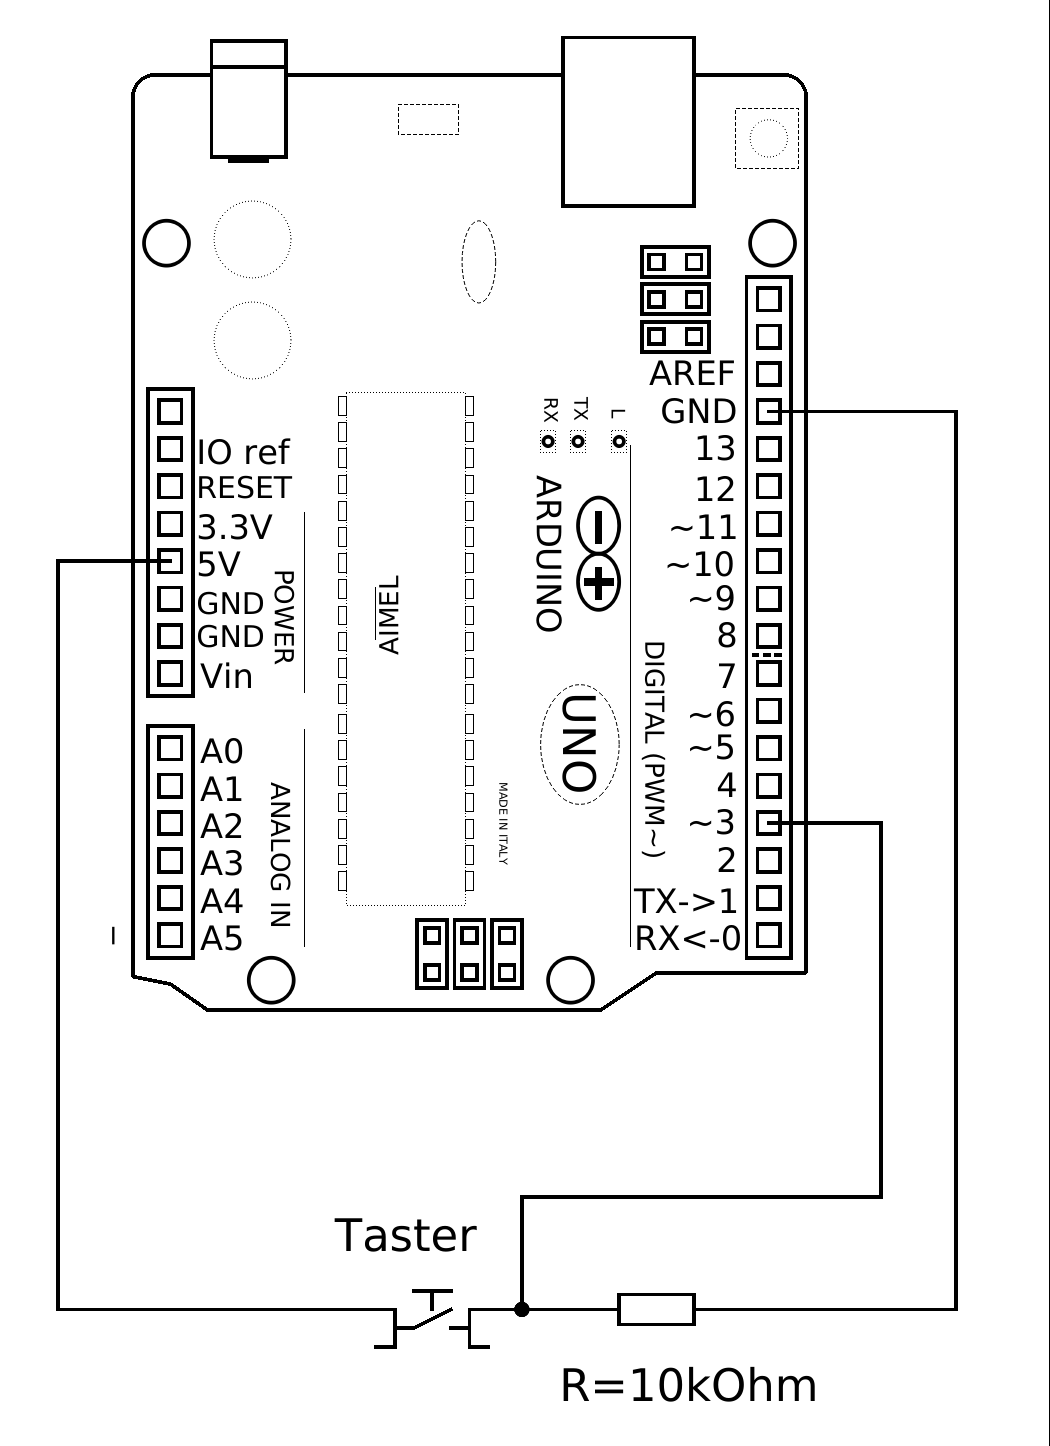
\includegraphics[width=0.8\textwidth]{Zeichnungen/taster-an-arduino.png}
		\caption{Taster offen (kein Stromfluss).}
	\end{minipage}
	\hfill
	\begin{minipage}{0.4\textwidth}
		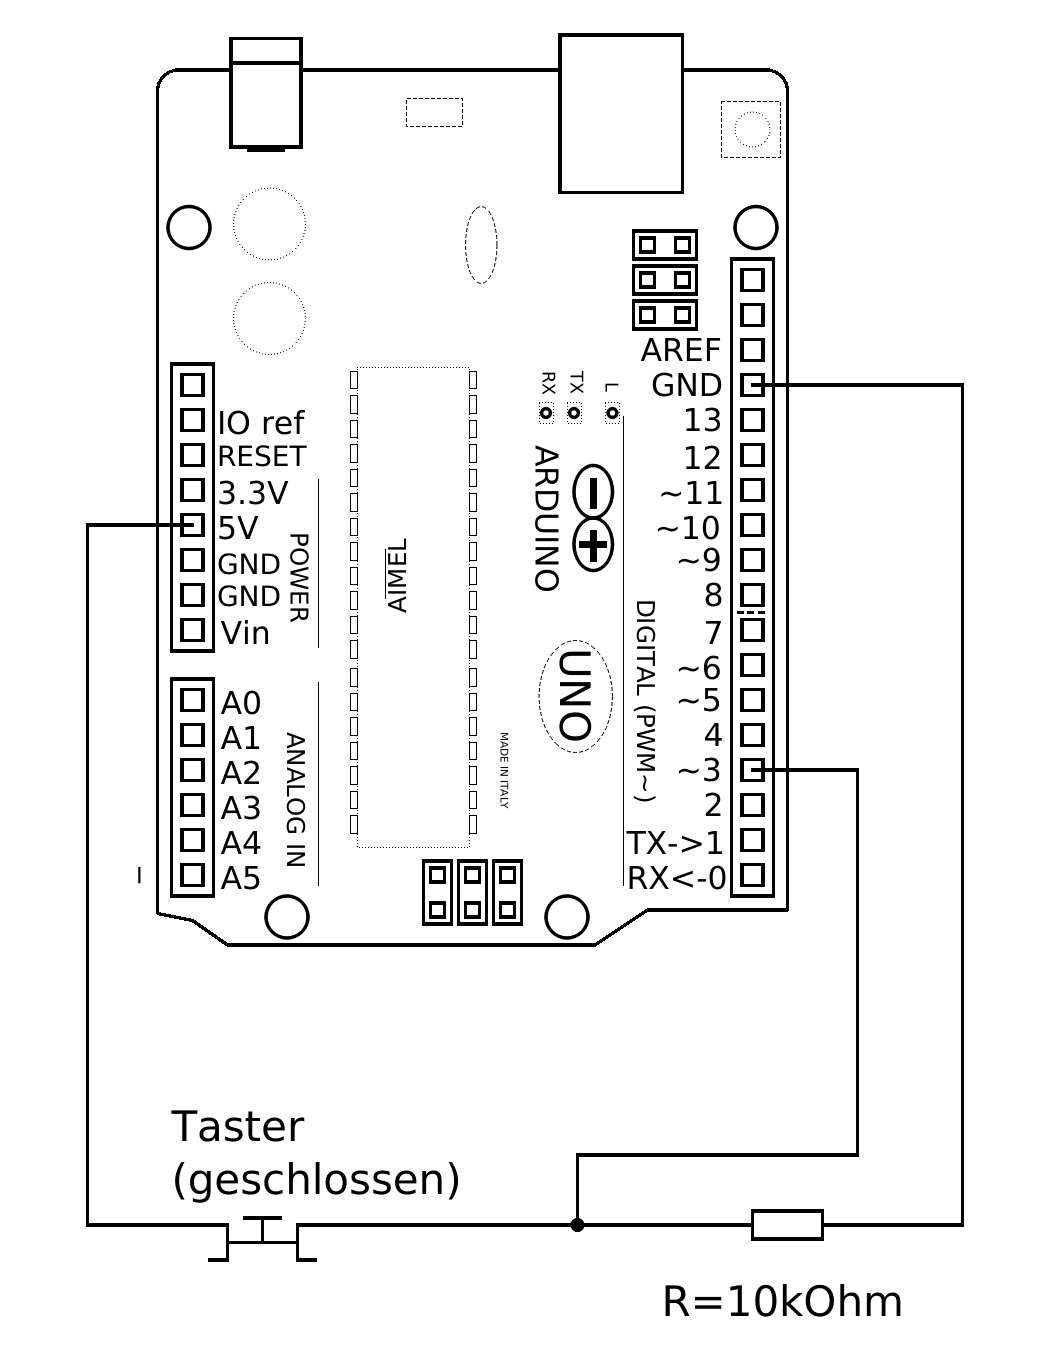
\includegraphics[width=0.8\textwidth]{Zeichnungen/taster-an-arduino-geschlossen.png}
		\caption{Taster geschlossen (Stromfluss).}
	\end{minipage}
	\hfill
	\label{abb:schaltplan-taster}
\end{figure}

\begin{zsfg}{Boolsche Werte einlesen} \label{sec:digitalread}
	Ein Potential von 5\,V wird im Programmcode auch als \texttt{HIGH}, \texttt{1} oder \texttt{TRUE} bezeichnet. Ein Potential von 0\,V wird im Programmcode auch als \texttt{LOW}, \texttt{0} oder \texttt{FALSE} bezeichnet. Ein digitaler Pin kann stets nur einen dieser beiden Zustände einnehmen. Potentiale von mehr als 1,4\,V werden stets als \texttt{HIGH} bzw. \texttt{TRUE} interpretiert.
	
	\begin{wrapfigure}{r}{0.25\textwidth}
		\centering
		
\includegraphics[width=0.25\textwidth]{pics/digitalread.png}
		\label{abb:digitalread}
	\end{wrapfigure}
	Dementsprechend hat der Befehl zum Einlesen des Potentials am digitalen Pin \emph{zwei mögliche Rückgabewerte}: \texttt{TRUE} oder \texttt{FALSE}. Das erkennt man auch an der eckigen Form das Befehls.
\end{zsfg}


\newpage
\begin{projekt}[Fußgängerampel]\label{proj:fussampel}
	\begin{wrapfigure}{r}{0.4\textwidth}
		\centering
		\vspace{-2\baselineskip}
		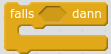
\includegraphics[width=0.15\textwidth]{pics/falls-dann.png}
		\label{abb:falls-dann}
	\end{wrapfigure}
	Baue und programmiere eine Fußgängerampel!
\end{projekt}
\marginpar{%
	\footnotesize%
	\werkzeug Neue \\
	Werkzeuge:\\
	\hyperref[sec:bewegungsmelder]{Bewegungs-\\melder}\\%
	\hyperref[sec:neigungsschalter]{Neigungs-\\schalter}
}

\begin{projekt}[Juke-Box]\label{proj:jukebox}
	\begin{wrapfigure}{r}{0.5\textwidth}
		\centering
		\vspace{-\baselineskip}
		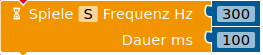
\includegraphics[width=0.5\textwidth]{pics/piezo-steuerung.png}
		\vspace{-\baselineskip}
		\label{abb:piezo-steuerung}
	\end{wrapfigure}
	Baue und programmiere eine Juke-Box!
	
	Die Juke-Box soll zwei verschiedene, kurze Melodien anspielen können.	
	(Zwei mögliche Beispiele mit Link zu den Noten: \href{https://www.lieder-archiv.de/alle\_meine\_entchen-notenblatt\_100055.html}{\enquote{Alle meine Entchen}}\footnote{\url{https://www.lieder-archiv.de/alle\_meine\_entchen-notenblatt\_100055.html}}, \href{https://www.lieder-archiv.de/o\_tannenbaum-notenblatt\_200078.html}{\enquote{Oh Tannenbaum}}\footnote{\url{https://www.lieder-archiv.de/o\_tannenbaum-notenblatt\_200078.html}}). 
	
	Dazu werden zwei Taster auf die beschriebene Art an zwei digitale Pins des Arduino angeschlossen. Schließe zudem an einen digitalen Pin einen Piezo-Summer an (siehe unten). 
	
	{\scriptsize Idee: Frick, Fritsch und Trick (2015): \emph{Einführung in Mikrocontroller - Der Arduino als Steuerzentrale}, Schülerforschungszentrum Bad Saulgau}
\end{projekt}

\begin{zsfg}{Piezo-Summer}

	\begin{minipage}{0.7\textwidth}
		Mit einem Piezo-Summer lassen sich Töne erzeugen, wenn man eine Spannung anschließt. Das lange Bein muss dabei an ein positives Potential angeschlossen werden; das kurze an ein negatives Potenzial bzw. GND. Ein Vorwiderstand ist dabei nicht notwendig, hilft aber die Lautstärke zu reduzieren.
	\end{minipage}
	\hfill
	\begin{minipage}{0.28\textwidth}
		\begin{minipage}{0.48\textwidth}
			\centering
			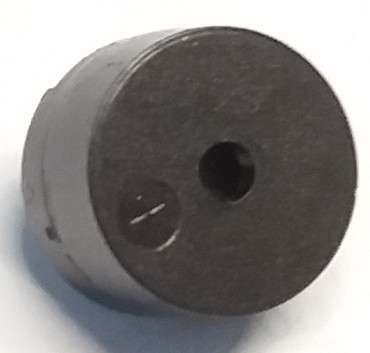
\includegraphics[width=0.9\textwidth]{./pics/piezo-summer.jpg}
		\end{minipage}
		\hfill
		\begin{minipage}{0.48\textwidth}
			\centering
			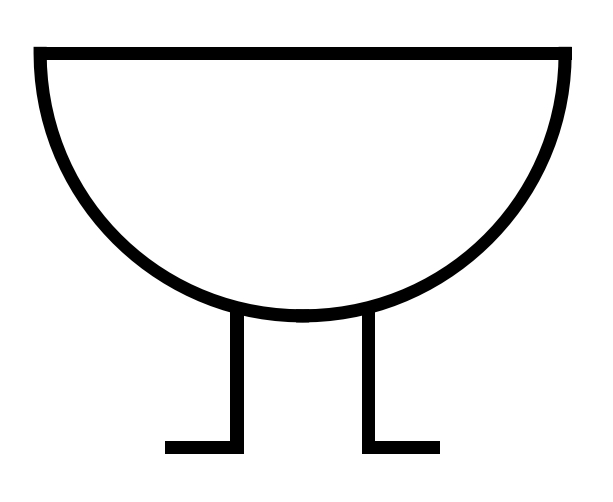
\includegraphics[width=\textwidth]{./pics/piezo-schaltsymbol.png}
		\end{minipage}
	\end{minipage}
	
	\bigskip
	\emph{Funktionsweise:}\label{piezo-effekt}
	
	\begin{wrapfigure}{r}{0.4\textwidth}
		\vspace{-\baselineskip}
		\centering
		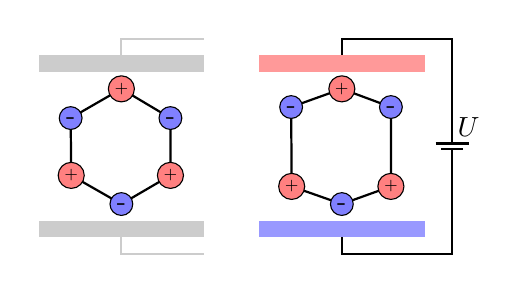
\begin{tikzpicture}[scale=0.7]
		\fill[white] (-0.2,-0.2) rectangle (8,4);
		%Kondensator links	
		\draw[gray!40,thick] (1.5,0.2) -- ++(0,-0.3) -- ++ (1.5,0);
		\fill[gray!40] (0,0.2) rectangle (3,0.5);
		\draw[gray!40,thick] (1.5,3.5) -- ++(0,0.3) -- ++ (1.5,0);
		\fill[gray!40] (0,3.2) rectangle (3,3.5);
		% Verbindungen/Sechseck
		\draw [thick] (1.5,0.8) -- (0.59,1.32) -- (0.58,2.36) -- (1.5,2.89) -- (2.39,2.36) -- (2.39,1.32) -- (1.5,0.8);
		%Ladungsverteilung
		\node at (1.5,0.8) [circle,fill=blue!50!white, draw, inner sep=1pt] (min1) {-};
		\node at (0.58,2.36) [circle,fill=blue!50!white, draw, inner sep=1pt] (min2) {-};
		\node at (2.39,2.36) [circle,fill=blue!50!white, draw, inner sep=1pt] (min3) {-};
		\node at (1.5,2.89) [circle,fill=red!50!white, draw, inner sep=1pt] (plus1) {\tiny +};
		\node at (0.59,1.32) [circle,fill=red!50!white, draw, inner sep=1pt] (plus2) {\tiny +};
		\node at (2.39,1.32) [circle,fill=red!50!white, draw, inner sep=1pt] (plus3) {\tiny +};
		%	
		%Kondensator rechts
		\draw[thick] (5.5,0.2) -- ++(0,-0.3) -- ++ (2,0) -- ++(0,1.9) ++(-0.2,0) -- ++(0.4,0);
		\fill[blue!40] (4,0.2) rectangle (7,0.5);
		\draw[thick] (5.5,3.5) -- ++(0,0.3) -- ++ (2,0) -- ++(0,-1.9) ++(-0.3,0) -- ++(0.6,0);
		\fill[red!40] (4,3.2) rectangle (7,3.5);
		\node at (7.8,2.2) {$U$};
		% Verbindungen/Sechseck rechts
		\draw [thick] (5.5,0.8) -- (4.59,1.12) -- (4.58,2.56) -- (5.5,2.89) -- (6.39,2.56) -- (6.39,1.12) -- (5.5,0.8);
		%Ladungsverteilung rechts
		\node at (5.5,0.8) [circle,fill=blue!50!white, draw, inner sep=1pt] (min11) {-};
		\node at (4.58,2.56) [circle,fill=blue!50!white, draw, inner sep=1pt] (min21) {-};
		\node at (6.39,2.56) [circle,fill=blue!50!white, draw, inner sep=1pt] (min31) {-};
		\node at (5.5,2.89) [circle,fill=red!50!white, draw, inner sep=1pt] (plus11) {\tiny +};
		\node at (4.59,1.12) [circle,fill=red!50!white, draw, inner sep=1pt] (plus21) {\tiny +};
		\node at (6.39,1.12) [circle,fill=red!50!white, draw, inner sep=1pt] (plus31) {\tiny +};
		\end{tikzpicture}
	\end{wrapfigure}
	In einem Piezo-Summer befindet sich ein Kristall mit unterschiedlichen Ladungsschwerpunkten, der von einem Kondensator umgeben ist. Wenn von außen an den Kristall eine Spannung angelegt wird, dann verformt sich die Kristallstruktur durch die Anziehung zwischen den Ladungsschwerpunkten und den Kondensatorplatten (\emph{\href{https://de.wikipedia.org/wiki/Piezoelektrizit\%C3\%A4t}{inverser piezo-elektrischer Effekt}}). Wenn keine Spannung anliegt, verformt sich der Kristall zurück. Durch diese Verformungen entstehen Druckwellen in der Luft, die wir als Ton wahrnehmen können.
\end{zsfg}
\vfill

\section{Vermischte Übungen}

\begin{aufgabe} \emph{Reihenschaltung}
	
	Eine rote LED soll an Pin 13 des Arduino betrieben werden. Durch die LED soll eine Stromstärke von $\SI{10}{\milli\ampere}$ fließen, was bei einer Spannung von $\SI{2,1}{\volt}$ an der LED der Fall ist. 
	\begin{enumerate}[label=\alph*), itemsep=0ex]
		\item Zeichne den zugehörigen Schaltplan.
		\item Berechne, wie groß der Vorwiderstand gewählt werden muss, damit diese Werte erreicht werden.
	\end{enumerate}
\end{aufgabe}

\begin{aufgabe} \emph{Parallelschaltung}
	
	Drei grüne LEDs sollen parallel geschaltet an Pin 13 des Arduino angeschlossen und mit einem gemeinsamen Vorwiderstand betrieben werden. Die LEDs halten eine Stromstärke von maximal $\SI{20}{\milli\ampere}$ bei einer Spannung von $\SI{3,3}{\volt}$ aus.
	
	\begin{enumerate}[label=\alph*), itemsep=0ex]
		\item Zeichne den zugehörigen Schaltplan.
		\item Ein Digitalpin am Arduino darf maximal mit einer Stromstärke von $\SI{40}{\milli\ampere}$ belastet werden. Berechne, welche Stromstärke dann maximal durch die einzelnen LEDs fließen darf.
		\item Der Tabelle unten kannst du den zugehörigen Spannungswert an den LEDs entnehmen. Berechne, wie groß der gemeinsame Vorwiderstand der LEDs sein muss, damit die in b) berechnete Stromstärke eingehalten wird.
		
		\begin{tabular}{c | c | c | c | c | c | c}
			\hline
			\textbf{Spannung U} & 3,03\,V & 3,07\,V & 3,1\,V & 3,13\,V & 3,16\,V & 3,19\,V \\ \hline
			\textbf{Stromstärke I} & 10\,mA & 11\,mA & 12\,mA & 13\,mA & 14\,mA & 15\,mA  \\ \hline
		\end{tabular}
	\end{enumerate}
\end{aufgabe}

\begin{aufgabe} \emph{Schaltung einer RGB-LED}
	
	\begin{wrapfigure}{r}{0.3\textwidth}
		\vspace{-\baselineskip}
		\centering
		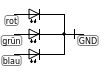
\includegraphics[width=0.2\textwidth]{./pics/rgb-led-schaltplan.png}
		\caption{Verschaltung der RGB-LED.}
		\vspace{-\baselineskip}
	\end{wrapfigure}
	Eine RGB-LED besteht aus drei einzelnen LEDs (rot, grün, blau), die jeweils über einen eigenen Digitalpin angesteuert werden (vgl. Schaltplan rechts). Am gemeinsamen GND-Anschluss soll ein gemeinsamer Vorwiderstand für alle LEDs angebracht werden, um die Stromstärke auf maximal $\SI{15}{\milli\ampere}$ zu begrenzen. Die Spannung an den LEDs sollte dann $\SI{2,25}{\volt}$ nicht überschreiten.
	\begin{enumerate}[label=\alph*), itemsep=0ex]
		\item Erkläre, welche Unterschiede zur Parallelschaltung von drei LEDs an \emph{einem} Digitalpin zu beachten sind.
		\item Berechne, wie groß der gemeinsame Vorwiderstand mindestens sein muss.
	\end{enumerate}
\end{aufgabe}

\newpage
\begin{aufgabe} \emph{Farbcodierung von Widerständen}
	
	\begin{enumerate}[label=\alph*), itemsep=0ex]
		\item Gib die Farbcodierung der folgenden Widerstandsgrößen an:
			\begin{multicols}{3}
				\begin{enumerate}[label=(\arabic*)]
					\item $\SI{330}{\ohm} \pm 1\%$,
					\item $\SI{10}{\kilo\ohm} \pm 2\%$,
					\item $\SI{4,7}{\kilo\ohm} \pm 10\%$.
				\end{enumerate}
			\end{multicols}
		\item Gib die Größe der folgenden Widerstände an:
			\begin{multicols}{2}
				\begin{enumerate}[label=(\arabic*)]
					\item 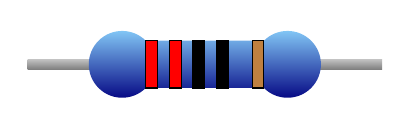
\begin{tikzpicture}[scale=0.3]
							\shade [top color=lightgray, bottom color=gray] (-5,0.8) rectangle (10,1.2);
							\shade [top color=LightSkyBlue, bottom color=NavyBlue] (0,0) -- (5,0) arc [start angle=-135, end angle=135, radius=1.414] -- (0,2) arc [start angle=45, end angle=315, radius=1.414];
							\draw [fill=red] (0,0) rectangle ++(0.5,2);
							\draw [fill=red] (1,0) rectangle ++(0.5,2);
							\draw [fill=black] (2,0) rectangle ++(0.5,2);
							\draw [fill=black] (3,0) rectangle ++(0.5,2);
							\draw [fill=brown] (4.5,0) rectangle ++(0.5,2);
						 \end{tikzpicture}
					\item 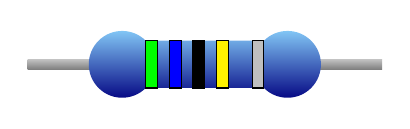
\begin{tikzpicture}[scale=0.3]
							\shade [top color=lightgray, bottom color=gray] (-5,0.8) rectangle (10,1.2);
							\shade [top color=LightSkyBlue, bottom color=NavyBlue] (0,0) -- (5,0) arc [start angle=-135, end angle=135, radius=1.414] -- (0,2) arc [start angle=45, end angle=315, radius=1.414];
							\draw [fill=green] (0,0) rectangle ++(0.5,2);
							\draw [fill=blue] (1,0) rectangle ++(0.5,2);
							\draw [fill=black] (2,0) rectangle ++(0.5,2);
							\draw [fill=yellow] (3,0) rectangle ++(0.5,2);
							\draw [fill=lightgray] (4.5,0) rectangle ++(0.5,2);
						 \end{tikzpicture}
				\end{enumerate}
			\end{multicols}
	\end{enumerate}
	\emph{Hinweis:} Als Hilfsmittel ist die Widerstandskarte aus den Boxen zugelassen.
\end{aufgabe}

\begin{aufgabe} \emph{Pullup-Widerstand}
	
	\begin{figure}[H]
		\centering
		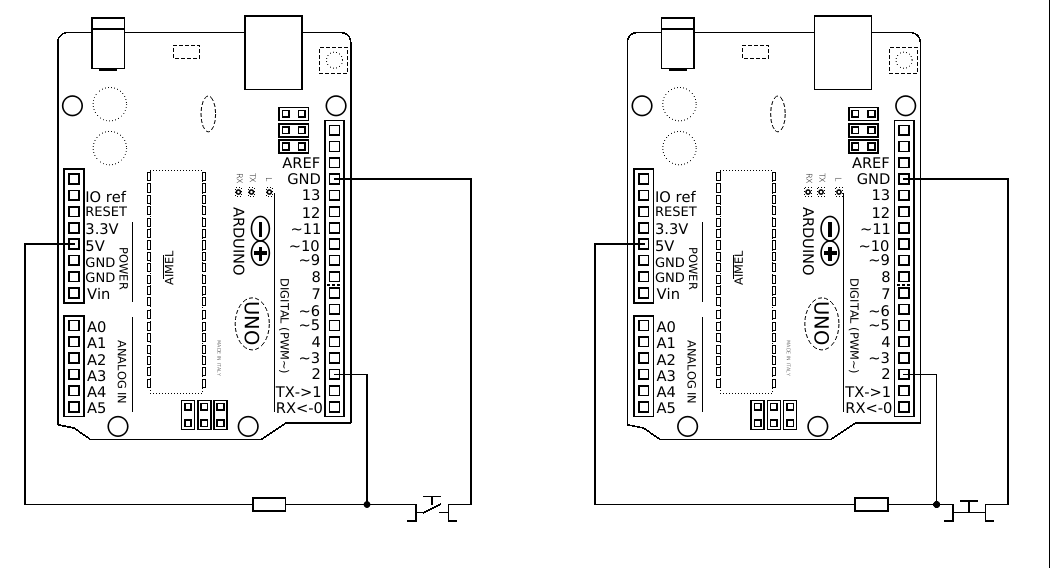
\includegraphics[width=0.8\textwidth]{./Zeichnungen/schaltplan-pullup.png}
	\end{figure}
	In der Abbildung wird ein Taster mit einem sogenannten Pullup-Widerstand an den Arduino angeschlossen. Links ist der Taster offen, rechts ist der Taster geschlossen.
	
	\bigskip
	\begin{minipage}{0.48\textwidth}
		\begin{enumerate}[label=\alph*), itemsep=0ex]
			\item Markiere die Kabel jeweils farbig, sodass die Kabel, die auf dem gleichen elektrischen Potential liegen, die gleiche Farbe haben. Notiere zudem den Wert des elektrischen Potentials.
			\item Erkläre, wie sich die Schaltung verhält, wenn das rechts abgebildete Programm auf dem Arduino läuft.
		\end{enumerate}
	\end{minipage}
	\hfill
	\begin{minipage}{0.5\textwidth}
		\centering
		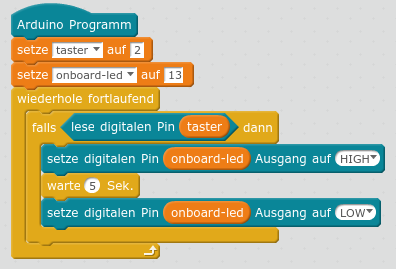
\includegraphics[width=0.9\textwidth]{./pics/programm-pullup-schaltung.png}
	\end{minipage}
\end{aufgabe}
\vfill


\begin{links}
	\item \href{https://www.youtube.com/watch?v=EbVmfGNwn0g}{FUTUREMAG}
	
	Kurze Dokumentation des FUTUREMAG zur Arduino-Welt
	
	\item \href{https://www.heise.de/make/meldung/Mehr-Komfort-der-Arduino-Ueberkopfwecker-4046184.html}{Arduino-Wecker}
	
	Mit einem selbst gebauten Wecker, der Uhrzeit und Alarmzeit getrennt voneinander anzeigt, erfüllte ein Bastler seinen Wunsch nach mehr Komfort.
	
	\item \href{https://www.instructables.com/id/Aquarium-LED-Controller/}{Aquarium-Licht}
	
	Der Bastler hinter diesem Projekt wollte seinen Fischen im Aquarium ein natürliches Licht einschließlich Sonnenaufgang, Sonnenuntergang und Nacht gönnen. Auf die gleiche Art und Weise kann man natürlich auch sein Terrarium beleuchten.
	
	\item \href{https://www.heise.de/make/meldung/Kein-Geld-fuer-eine-Oculus-Rift-VR-Brille-selbstgebaut-3949507.html}{VR-Brille}
	
	Drei Schüler aus Frankreich hatten kein Geld für eine Virtual Reality Brille – aber dafür das Know How, um sich mit einem Arduino und einem Gehäuse aus dem 3D-Drucker selbst eine VR-Brille zu basteln.
\end{links}